%%outline%% ECAL Cluster Calibration using Boosted Decision Tree

intro..
 talk about ECAL.
 introduce clustering algorithm in ECAL.
 HLT vs offline PF ECAL cluster

 expand more on:
  the PF cluster calibration.
  how it was done perviously, and now in this thesis.

computational details..
 3.1 Boosted Decision Tree (BDT)
  based semi-parametric regression.

 3.2 BDT training details
  samples being used. for training and validation.
  Calibration procedure. Input and target variables to BDT.

 3.3 fitting function
 Crystal Ball (CB) double function

Results and Discussion (might be moved to its chapter before conclusion)
 compare old vs new corrections
 check the response, resolution in each regions EE. EB. add comments if the results has improved or stayed the same.

%plots : showing (EB , EE regions)
%-  mu vs pt (covering 3 ranges of pt gen particle) (EB , EE regions)
%-  mu vs eta (for each range of pt) (EB region)


%\frame{
\begin{figure}
%\begin{verbatim}
%\end{verbatim}
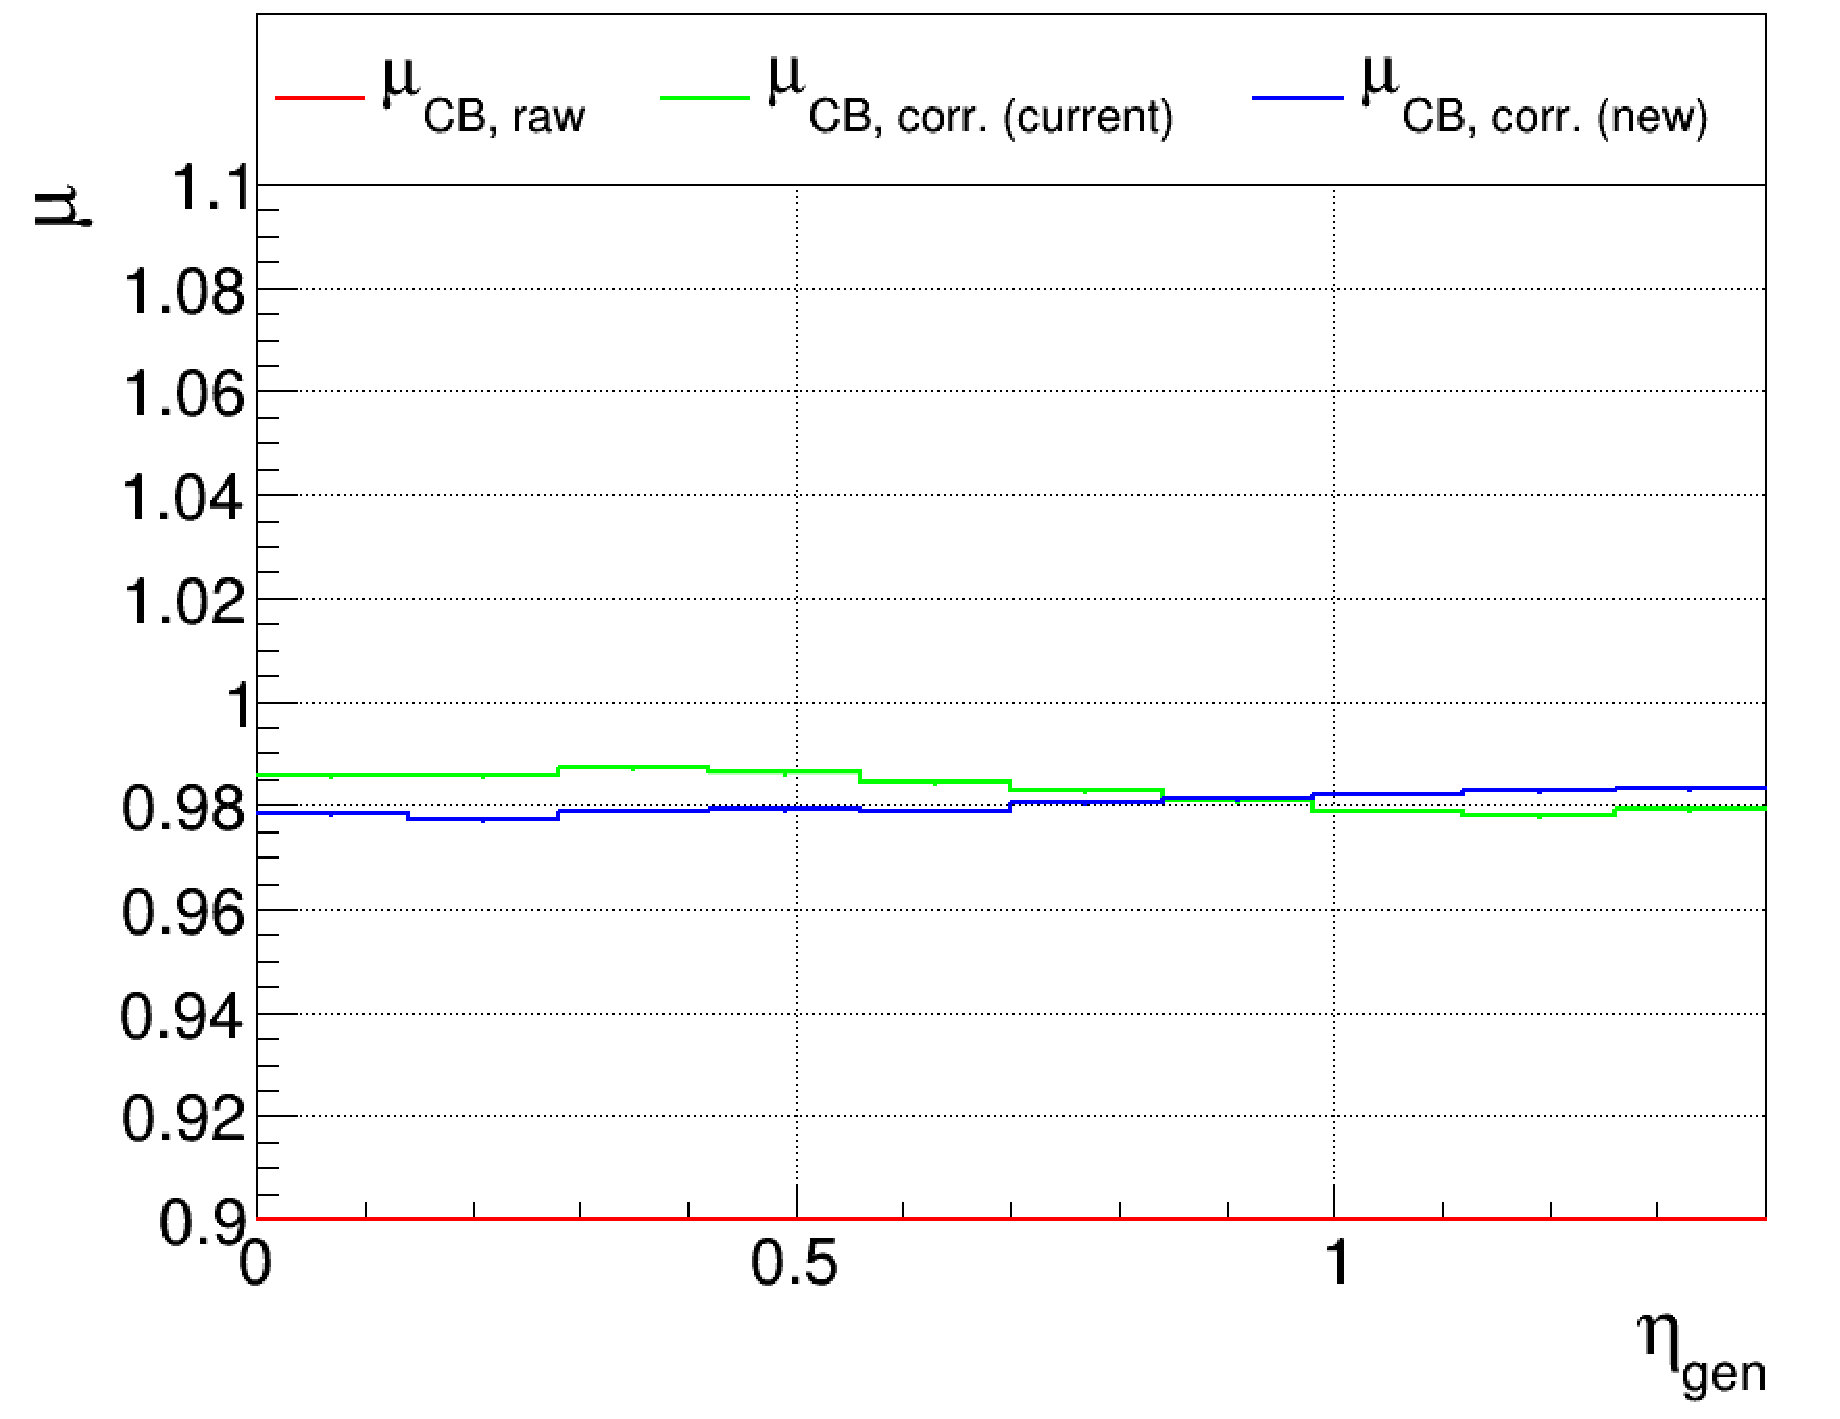
\includegraphics[width=0.495\textwidth]{./ECAL_plots/plotsPU/EB/FULL/pdf/EBFULL_GENETA_0005_0020_MuOverBins.pdf}
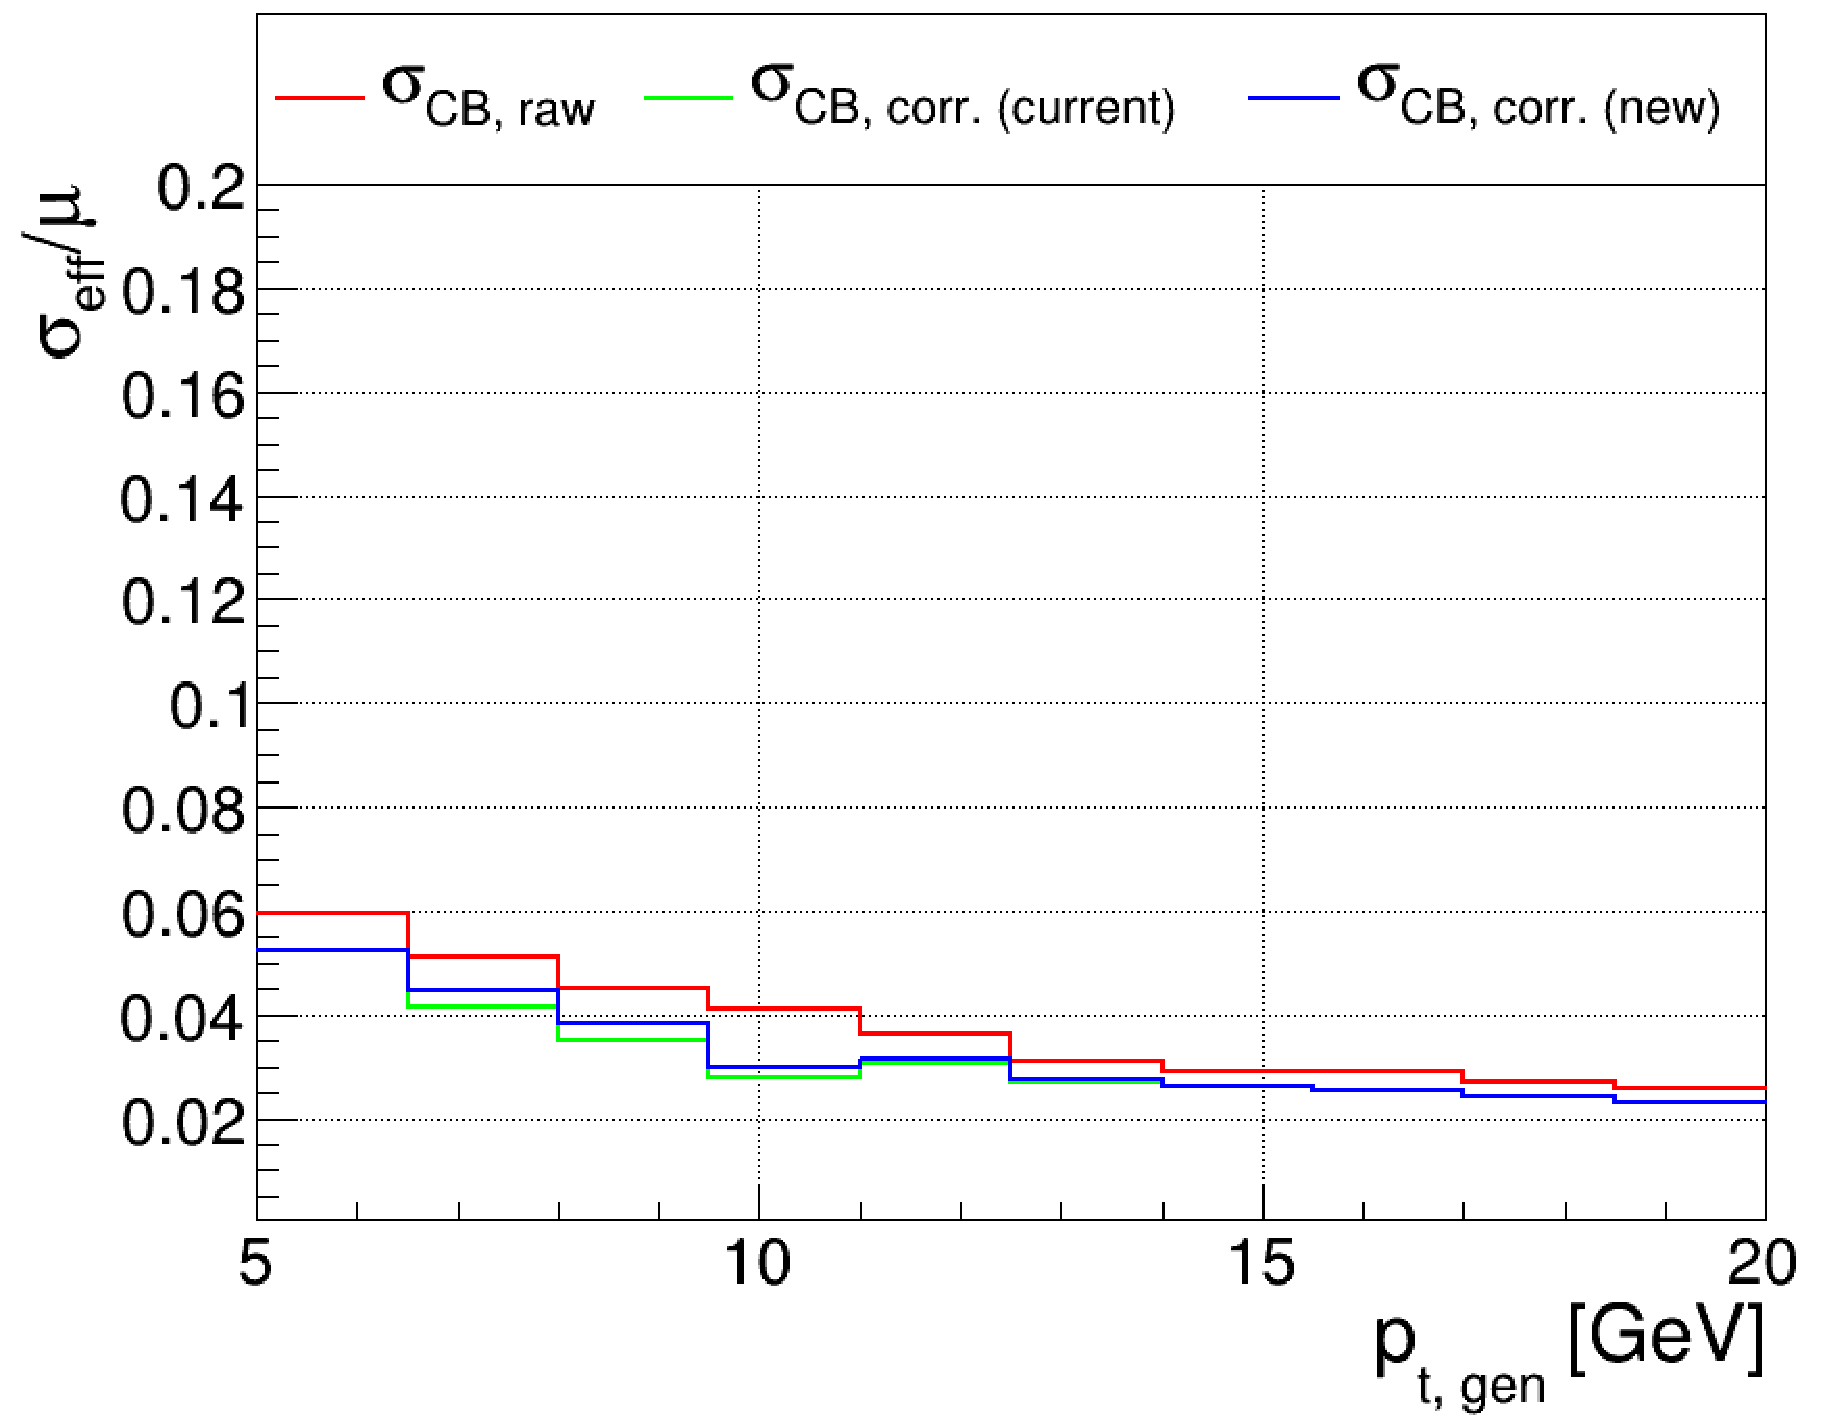
\includegraphics[width=0.495\textwidth]{./ECAL_plots/plotsPU/EB/FULL/pdf/EBFULL_GENPT_0005_0020_EffSigmaOverBins.pdf}
\caption{EB - Full Readout : mu vs eta}
\end{figure}
%}





Include some set of stamp plots. (where we get mu \& std from after fitting)

Now, for ZS set vs pt.


HLT vs offline PF ECAL cluster

%1-plots :
%- (PF cluster offline E / PFC online E) vs pt
%- (PF cluster offline E / PFC online E) vs eta
%%%%%%%%%%%%%%%%%%%%%%%%%%%%%%%%%%%%%%%%%%%%%%%
\begin{figure}
\caption{(PF cluster offline E / PFC online E) vs pt}
\end{figure}
\begin{figure}
\caption{(PF cluster offline E / PFC online E) vs eta}
\end{figure}


%%%%%%%%%%%%%%%%%%%%%%%%%%%%%%%%%%%%%%%%%%%%%%%%
%plots :
%- (PF cluster offline corrected E / PFC online corrected  E) vs pt
%- (PF cluster offline corrected E / PFC online corrected  E) vs eta
%%%%%%%%%%%%%%%%%%%%%%%%%%%%%%%%%%%%%%%%%%%%%%%
\begin{figure}
\caption{(PF cluster offline corrected E / PFC online corrected E) vs pt}
\end{figure}
\begin{figure}
\caption{(PF cluster offline corrected E / PFC online corrected E) vs eta}
\end{figure}
%%%%%%%%%%%%%%%%%%%%%%%%%%%%%%%%%%%%%%%%%%%%%%%%

\section{Footnotes}

Ut vitae elit blandit, dictum augue aliquam, dictum neque. Integer sit amet eros
iaculis, interdum est quis, convallis metus. Maecenas vestibulum id lectus at
pellentesque.\footnote{This is a short footnote.} Aliquam dignissim, turpis eget
hendrerit ullamcorper, magna magna consectetur odio, pulvinar vestibulum felis
enim in ipsum. Donec cursus pharetra fringilla. Integer placerat ultrices libero
non porta. In id orci in ipsum aliquet rhoncus. Fusce ornare ornare
volutpat.\footnote{And this is a rather longer footnote that requires more than
one line, demonstrating the required single spacing.}

Vivamus vel tortor vel nibh aliquet egestas. Nullam rutrum porttitor placerat.
Pellentesque mattis ullamcorper sollicitudin. Nam et arcu nisi. Aenean hendrerit
odio non nisi ultricies, in consectetur odio rhoncus. Donec cursus consequat
tincidunt. Morbi pellentesque ut sem sit amet sollicitudin. Quisque bibendum
tincidunt quam, eu condimentum dui ullamcorper at.

\section{Citations}

Here is a citation \cite{fake1}, and here is another \cite{fake2}. Citations are
nice. Depending on your choice of bibliography, there may be different formats
you can use. For example, Chicago provides a family of short citation commands.
